\begin{figure*}[t]
\begin{center}
\bgroup 
 %\def\arraystretch{0.2} 
 %\setlength\tabcolsep{0.2}
\begin{tabular}{cccc}
\subfloat[][]{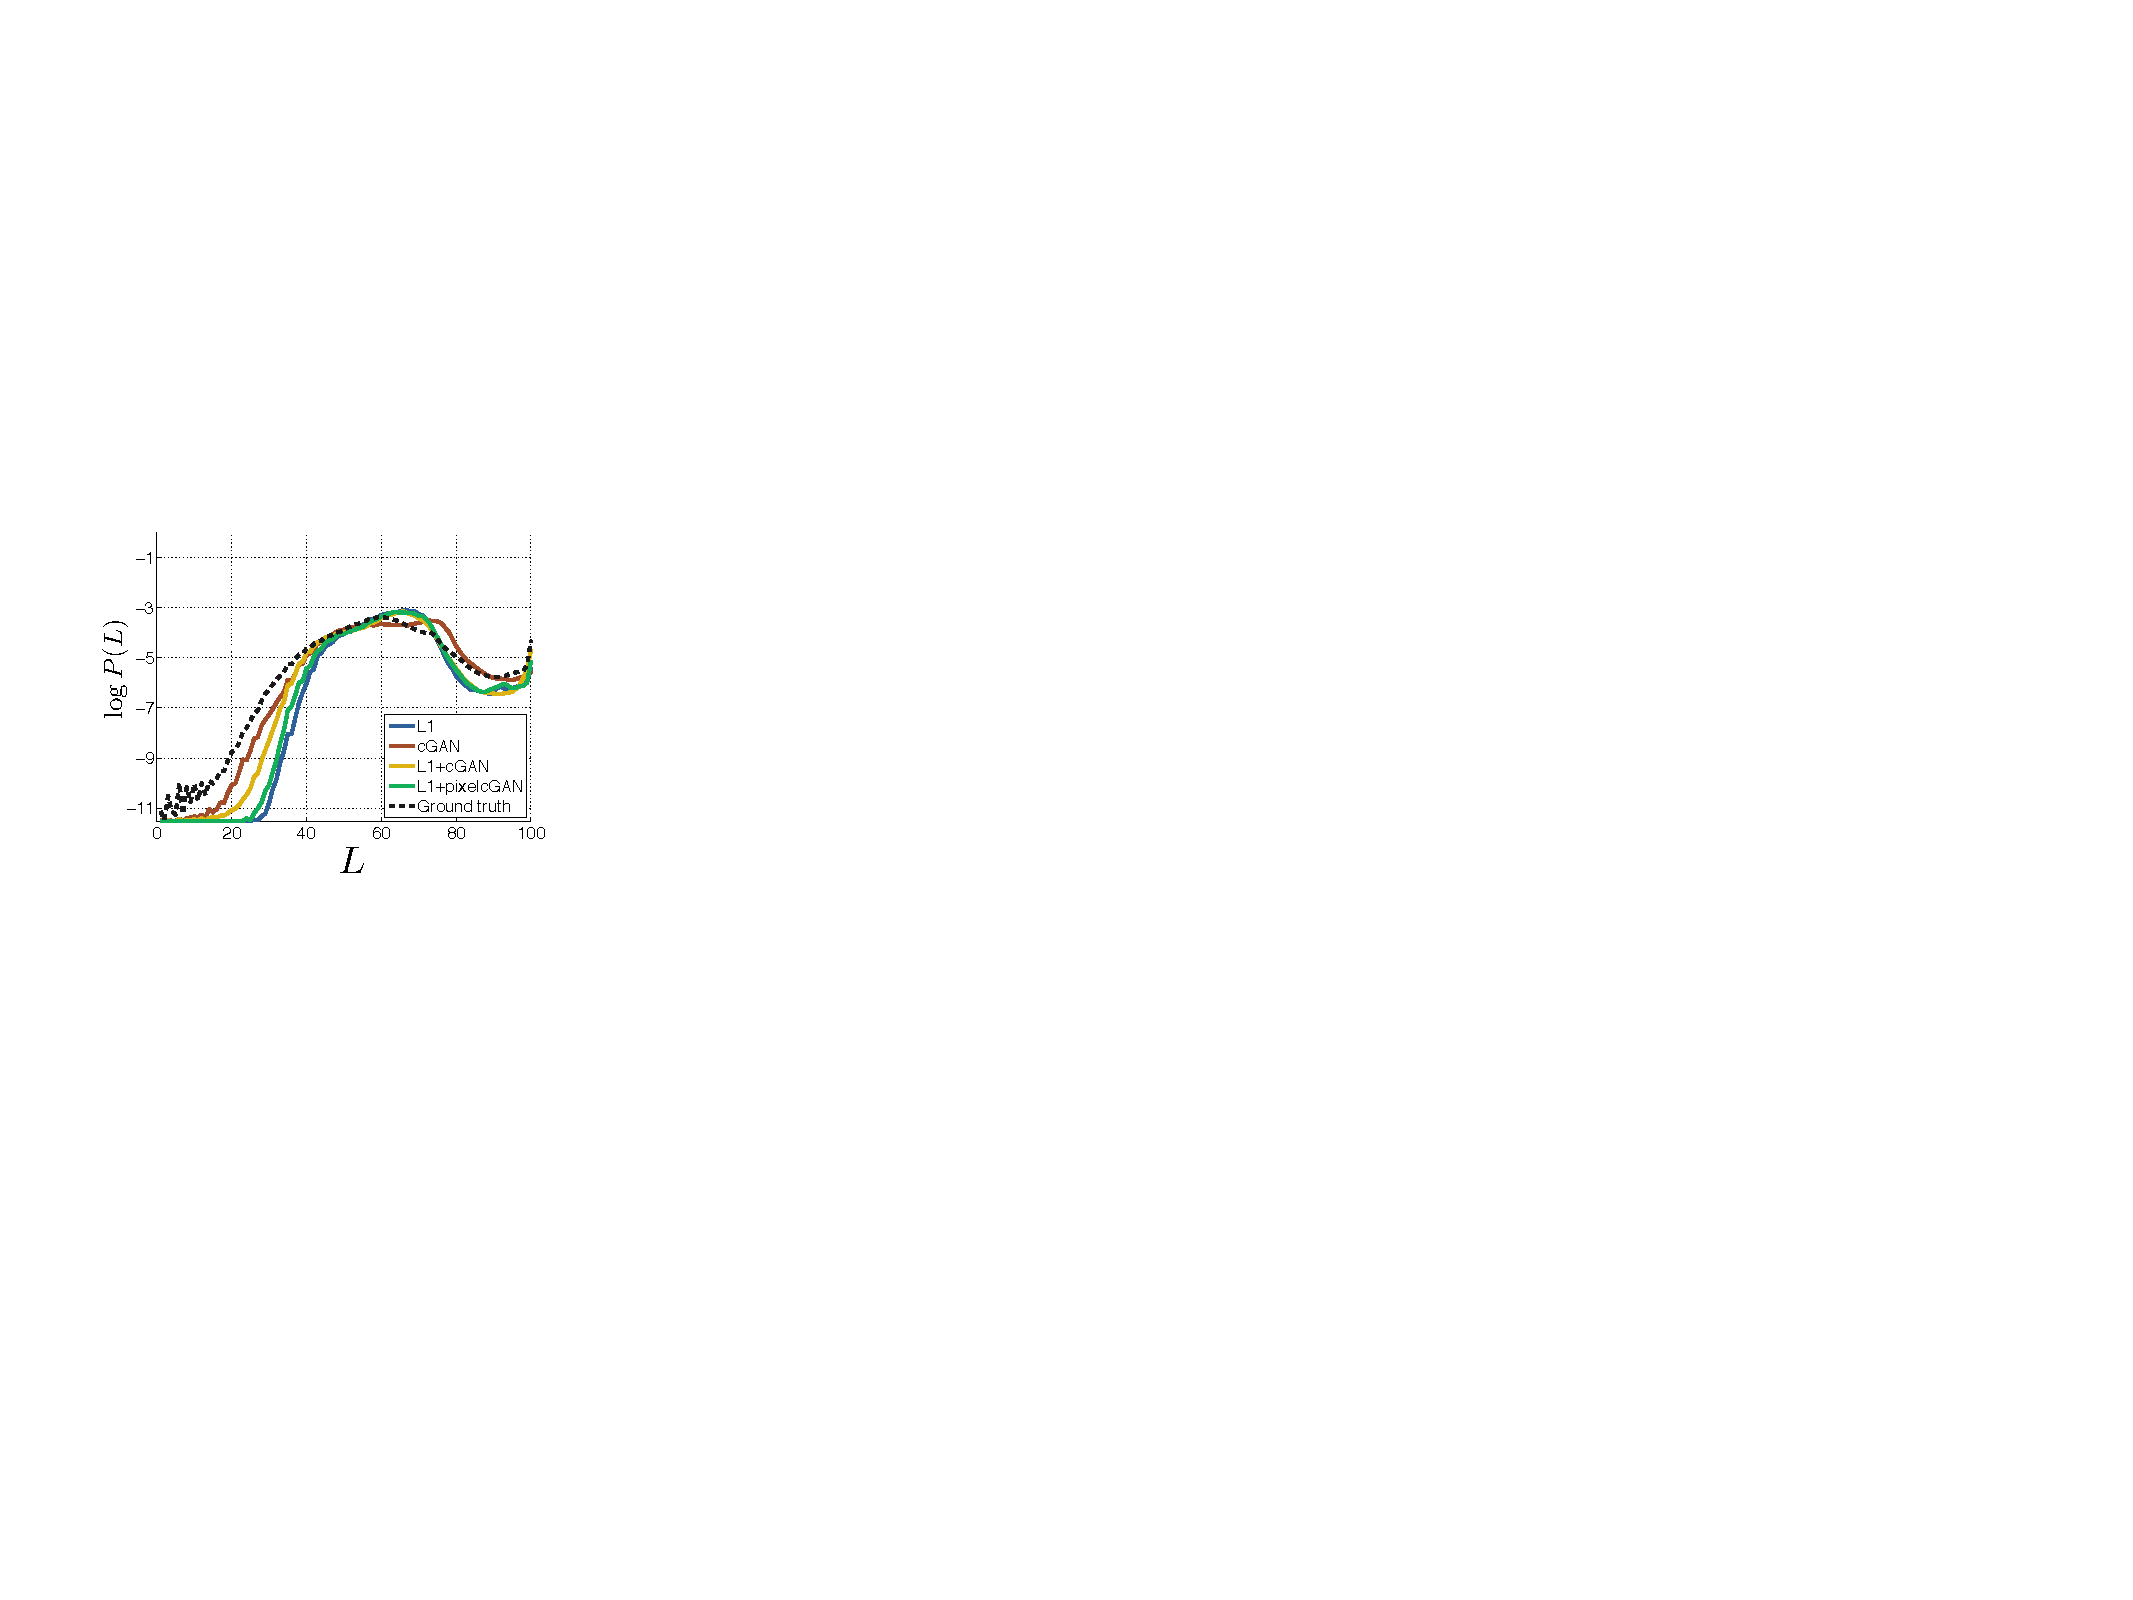
\includegraphics[width=0.2\linewidth]{figs/L_hists.pdf}} &
\subfloat[][]{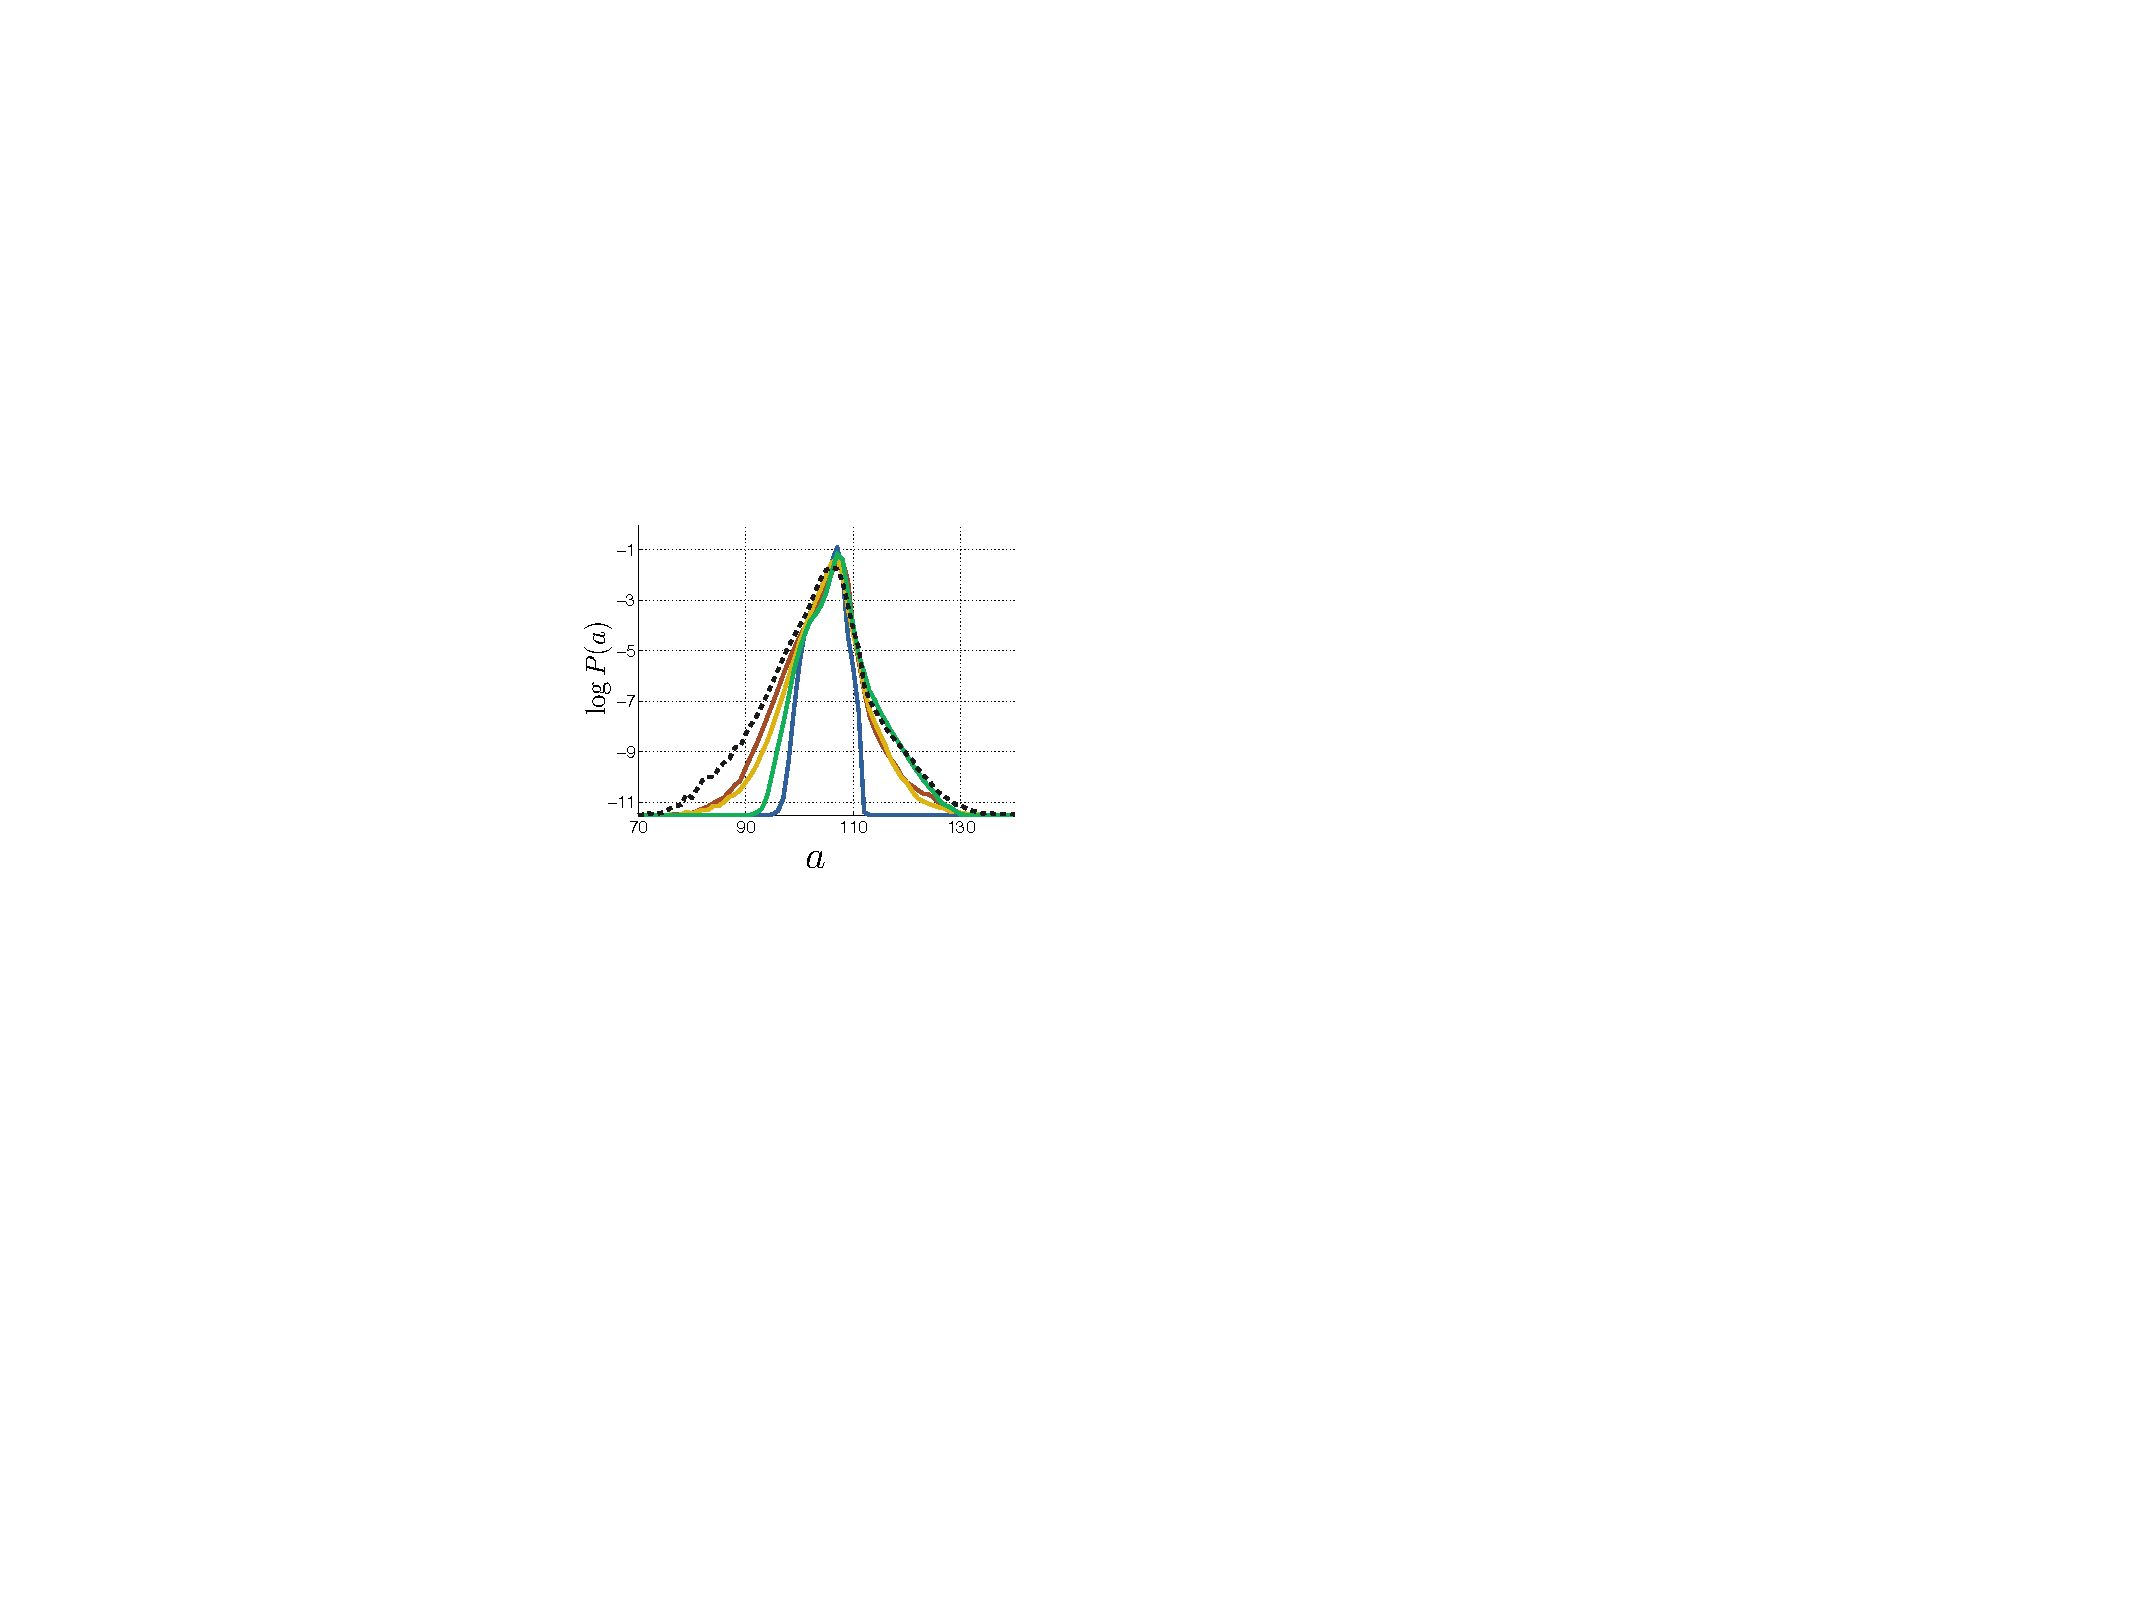
\includegraphics[width=0.2\linewidth]{figs/a_hists.pdf}} &
\subfloat[][]{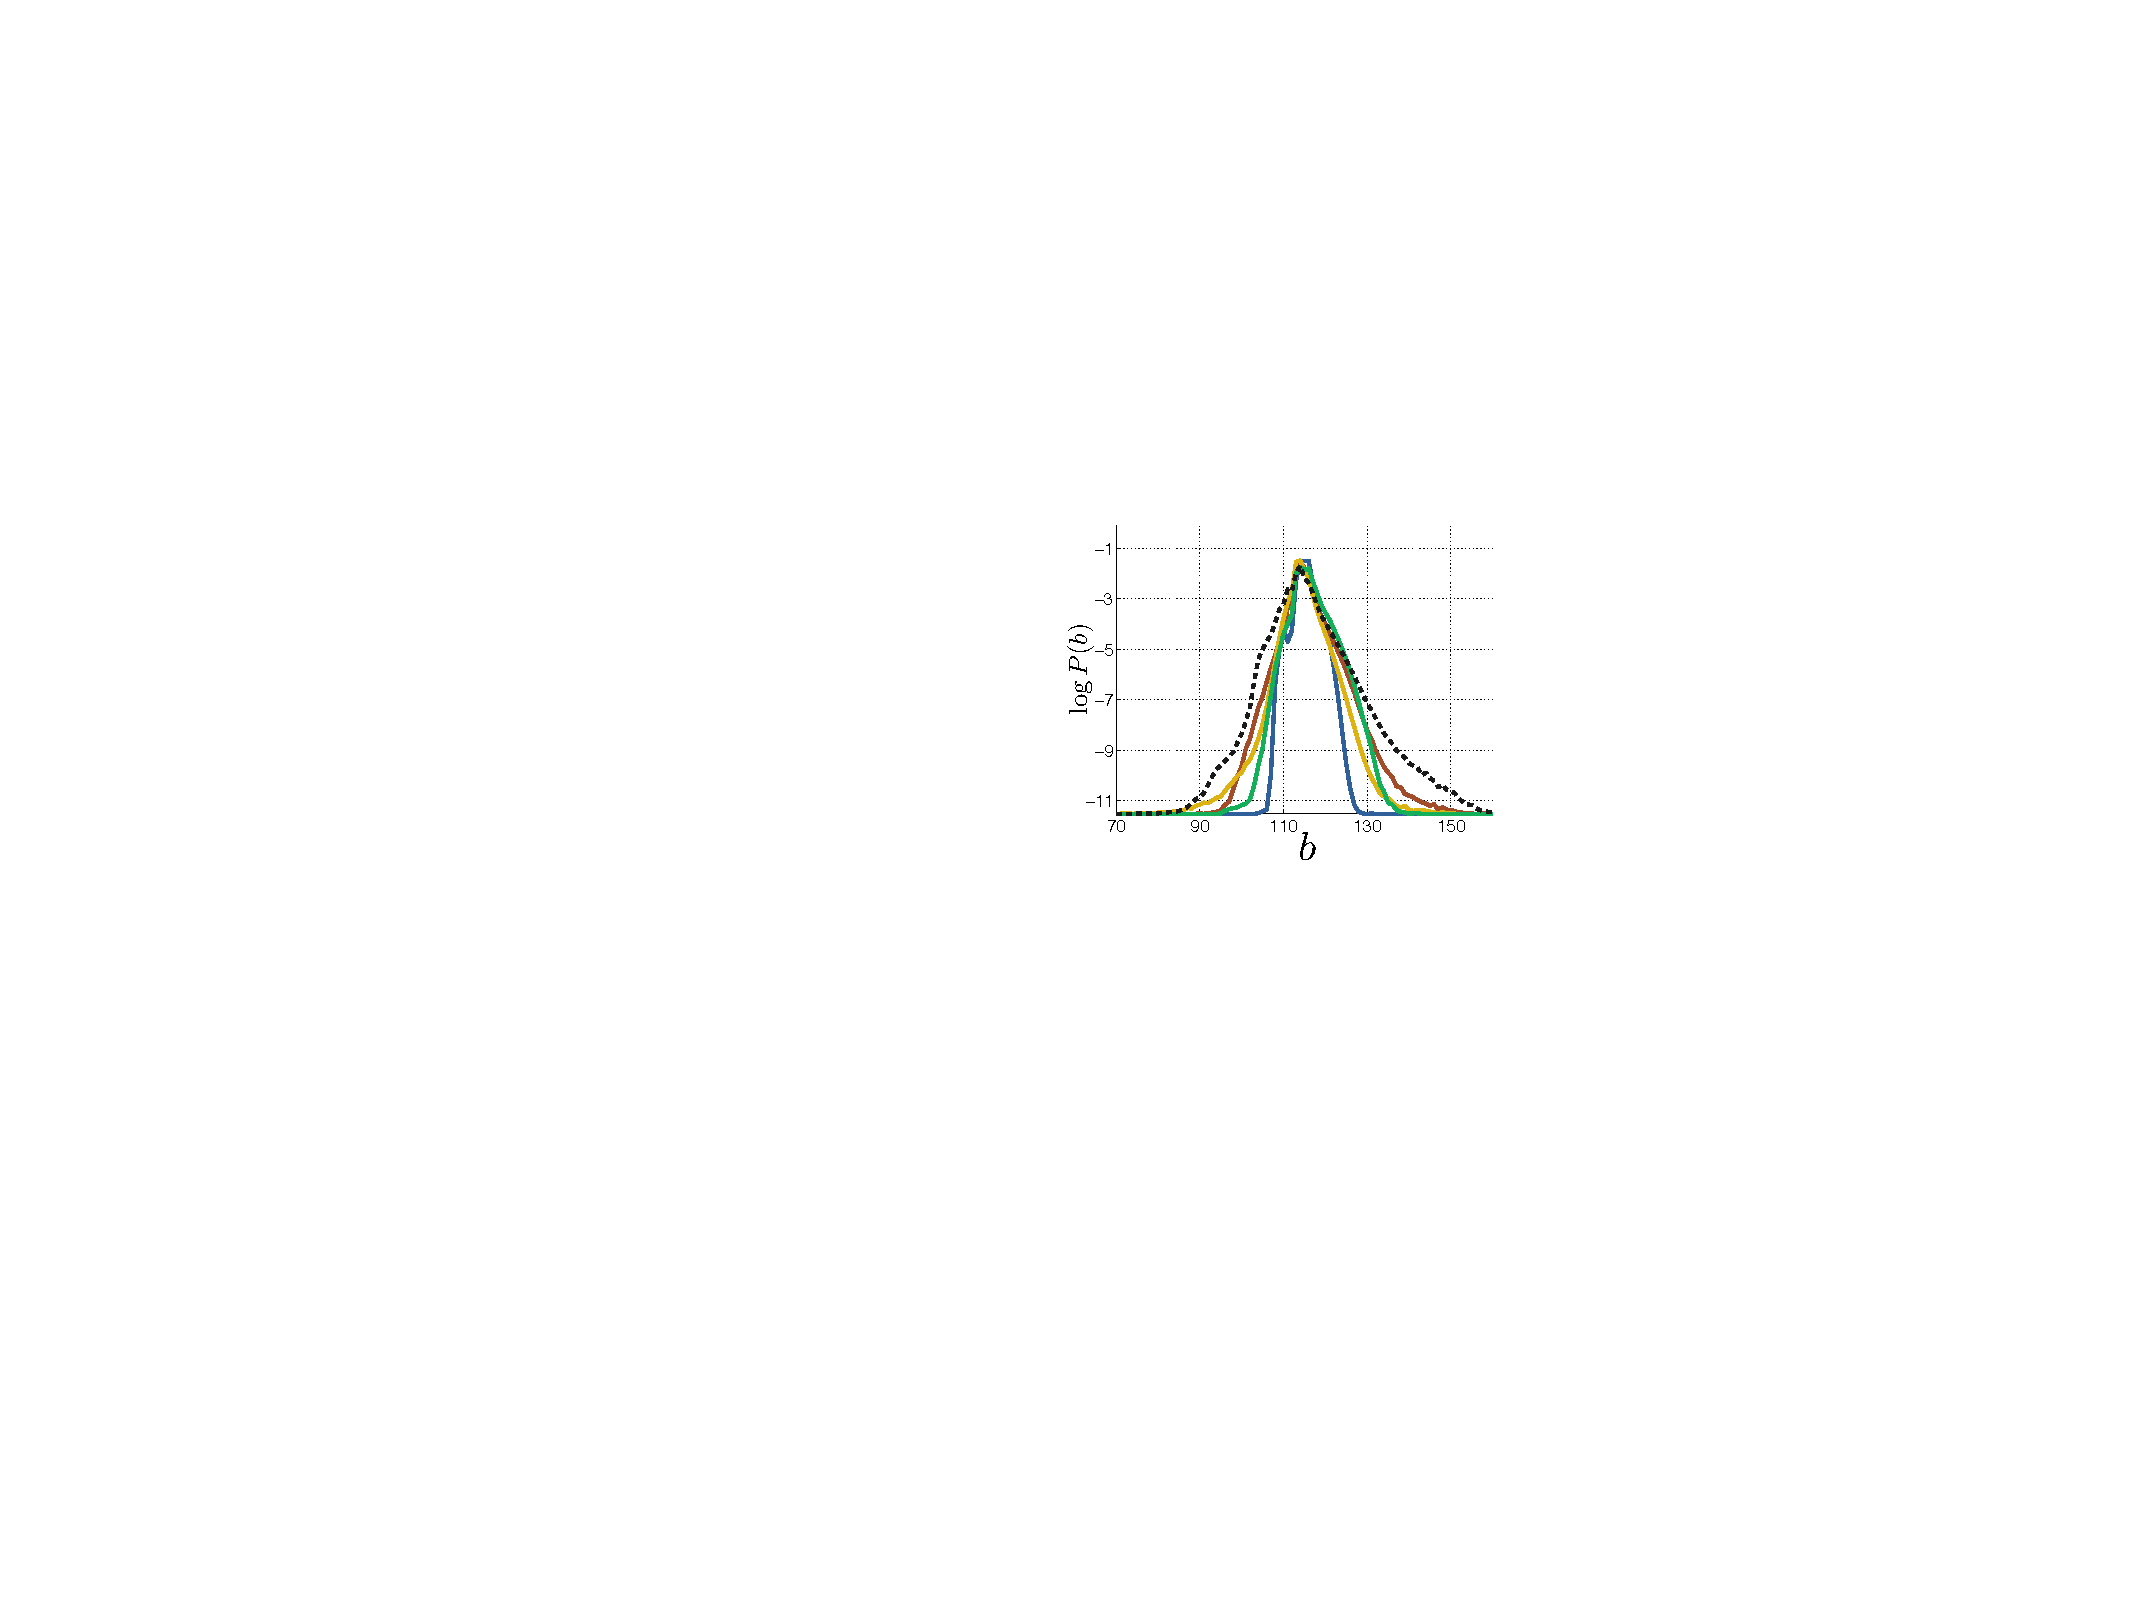
\includegraphics[width=0.2\linewidth]{figs/b_hists.pdf}} &

%\multicolumn{3}{c}{
\subfloat[][]{
\centering
\scalebox{0.75} {
\begin{tabular}[b]{lccccc}
& \multicolumn{3}{c}{Histogram intersection} \\
& \multicolumn{3}{c}{against ground truth} \\
\textbf{Loss} & L & a & b \\ \hline
\textbf{L1} & 0.81 & 0.69 & 0.70 \\
\textbf{cGAN} & \textbf{0.87} & 0.74 & \textbf{0.84} \\
\textbf{L1+cGAN} & 0.86 & \textbf{0.84} & 0.82 \\
\hline
\textbf{PixelGAN} & 0.83 & 0.68 & 0.78 
\end{tabular} }
\label{tab:color_hists}
}
%}

\end{tabular} \egroup 
\end{center}
\vspace{-0.2in}
\caption{Color distribution matching property of the cGAN, tested on Cityscapes. (c.f. Figure 1 of the original GAN paper \cite{goodfellow2014generative}). Note that the histogram intersection scores are dominated by differences in the high probability region, which are imperceptible in the plots, which show log probability and therefore emphasize differences in the low probability regions.}
\label{color_hists}
\end{figure*}